\chapter{Architettura}                %crea il capitolo
%%%%%%%%%%%%%%%%%%%%%%%%%%%%%%%%%%%%%%%%%imposta l'intestazione di pagina
\lhead[\fancyplain{}{\bfseries\thepage}]{\fancyplain{}{\bfseries\rightmark}}


L'applicazione è stata realizzata per la piattaforma mobile Android utilizzando il linguaggio di programmazione Kotlin, e altre librerie open-source.\\
Lo sviluppo della parte client si basa sul pattern Model View Presenter (MVP) e l'organizzazone dei file segue le classiche direttive di Android, differenziando quindi Activity, Fragment, Adapter e Servizi.\\
Il client quando richiede dei dati al database memorizza la risposta all'interno delle cache, in modo da consentire all'utente di interagire con l'applicazione anche in modalità offline, senza quindi necessitare di una connessione ad internet. Quando l'utente riacquisterà la connessione, tutti i cambiamenti apportati offline verranno inviati al database FireStore che si occuperà di risolvere eventuali conflitti, ed aggiornare il database e le cache del client attraverso l'SDK.\\
La parte server invece è stata realizzata utilizzando come BaaS Firebase e i suoi servizi per la gestone del database, autenticazione, notifiche e lo storage. Ogni servizio offerto da Firebase interagisce in maniera diretta o indiretta con tutti gli altri servizi, facilitando la gestisce dell'autenticazione, del database e dello storage online.\\


\newpage



\section{Architettura Firebase}                 %crea la sezione
La gestione del backend è stata realizzata utilizzando la piattaforma Firebase e i suoi servizi.
I servizi utilizzati per la gestione del backend sono:
\begin{enumerate}
\item \textbf{Auth}: Servizio per gestire l'autenticazione degli utenti
\item \textbf{Firestore}: Database real-time per la memorizzazione di tutti i dati utilizzati dall'applicazione.
\item \textbf{Storage}: Spazio di archiviazione utilizzato per salvare gli avatar degli utenti e le immagini dei gruppi.
\item \textbf{Cloud Functions}: Servizio utilizzato per monitorare i cambiamenti all'interno del database Firestore.
\item \textbf{Cloud Messaging}: Servizio utilizzato per gestire ed inviare notifiche ai dispositivi.
\end{enumerate}


\begin{figure}[!hb]
  \centering
  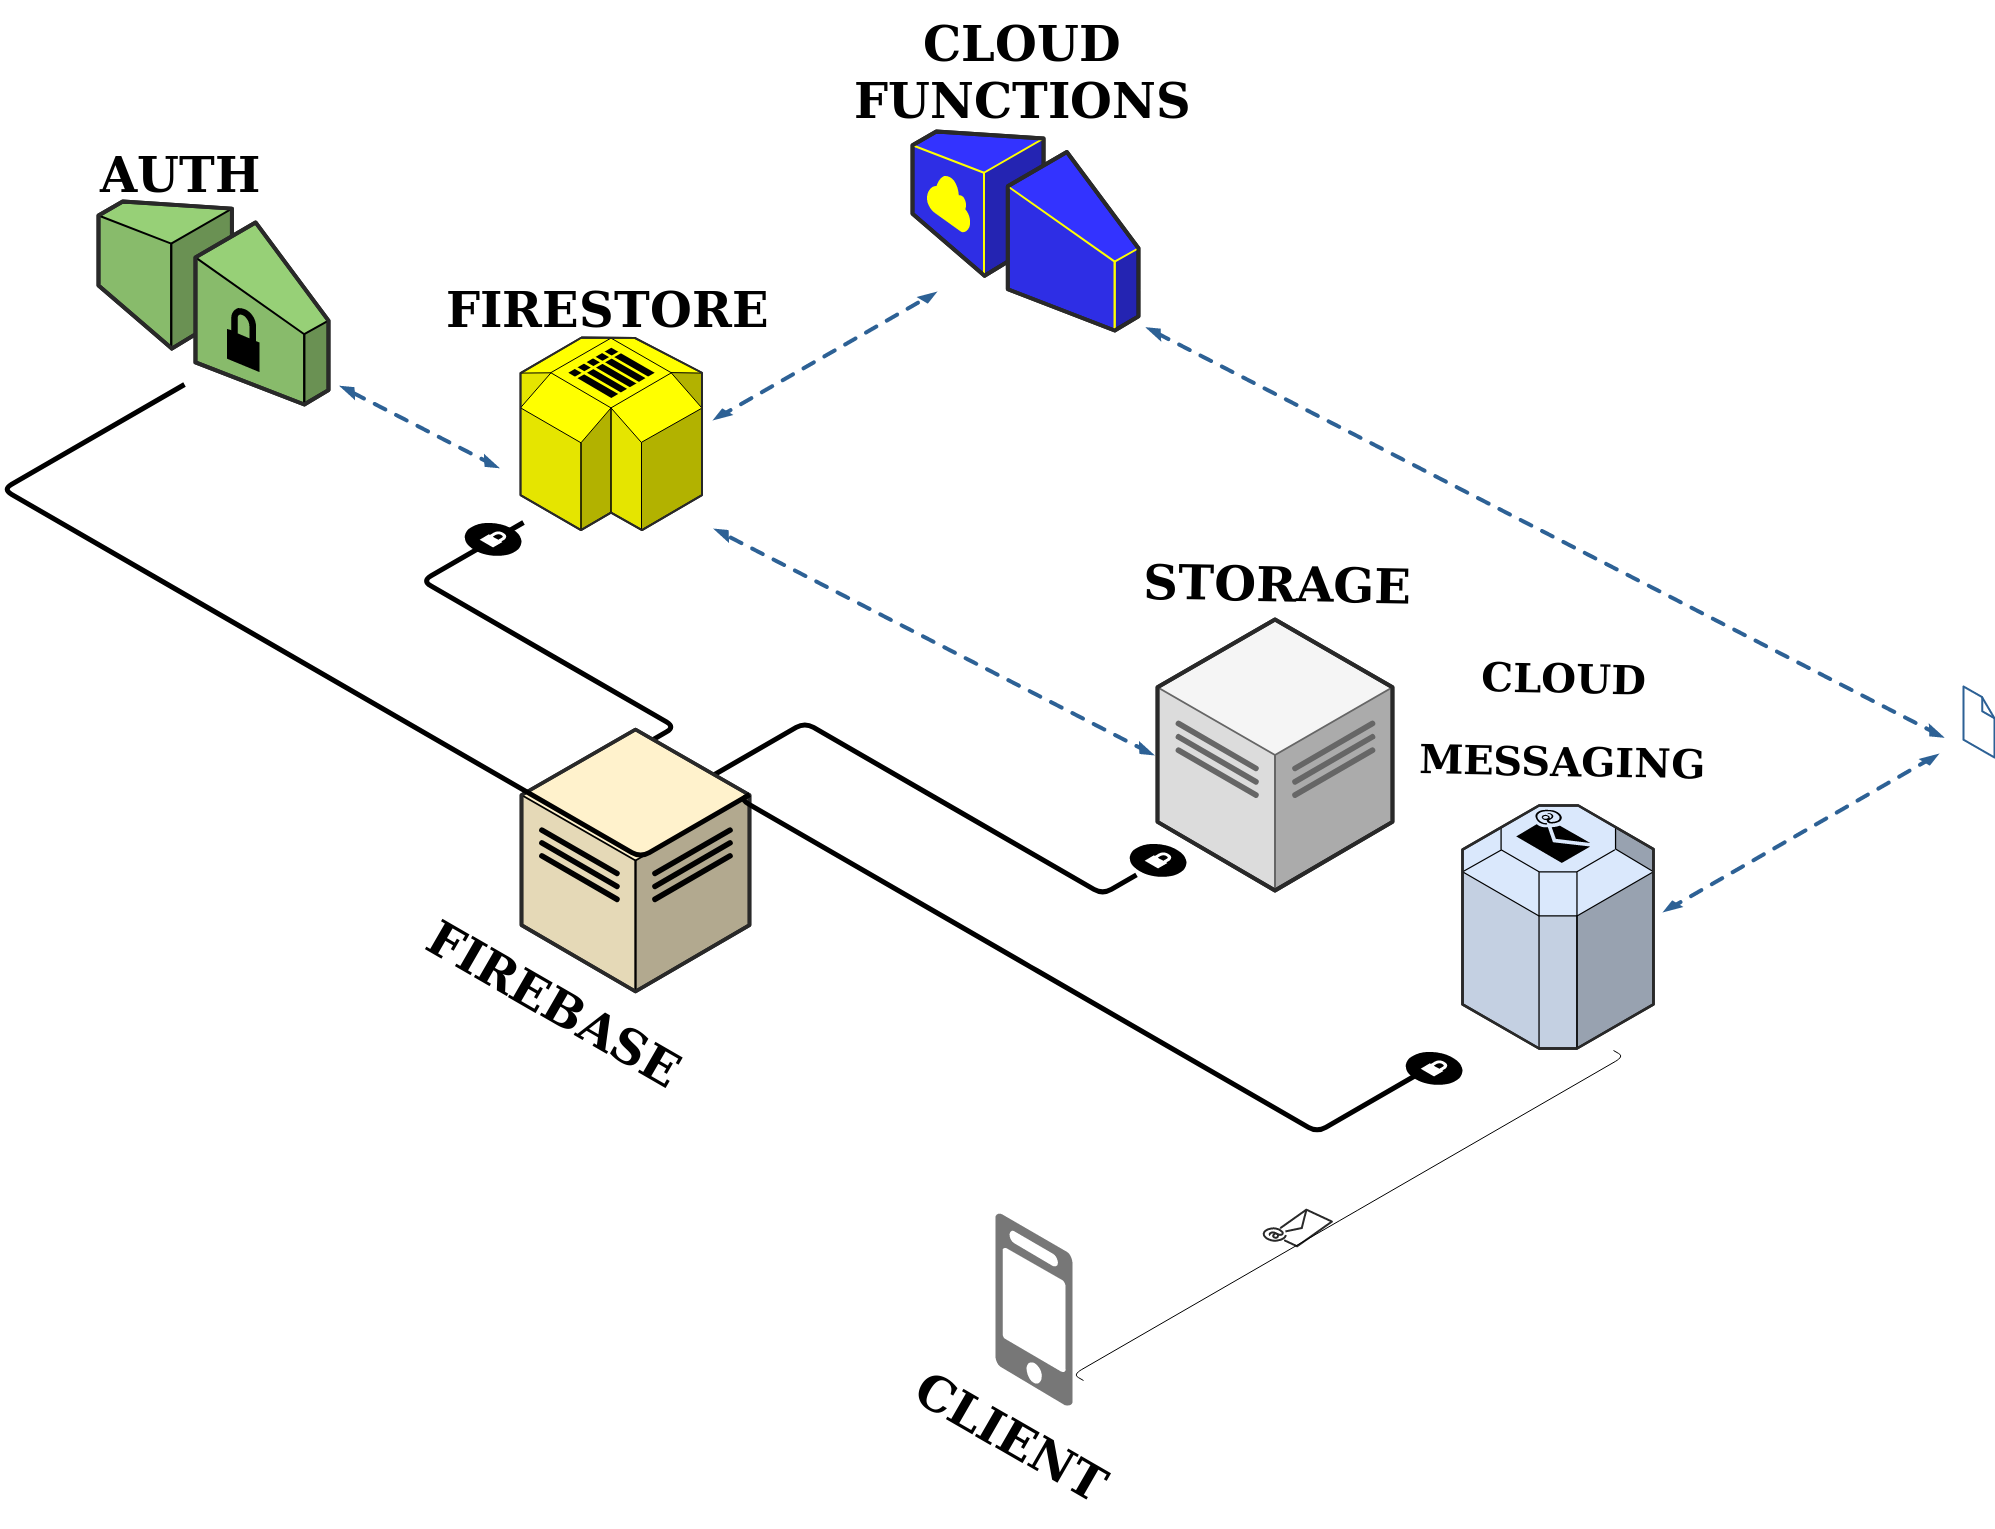
\includegraphics[width=0.8\textwidth]{immagini/server_arch.png}
  \caption{Architettura del server}\label{fig:Architettura del Server}
\end{figure}

\subsection{Autenticazione}
I client connessi a Firebase, hanno la possibilità di registrarsi attraverso email e social login (Google,Faceook,Twitter). Una volta effettuata la registrazione, FirebaseAuth assegnerà un identificativo univoco al nuovo client, memorizzando nei suoi server le informazioni basilari, quali: ID, nome, data di creazione, ultimo accesso, email e provider (Email, Google, Faceook, Twitter).
\begin{figure}[!h]
  \centering
  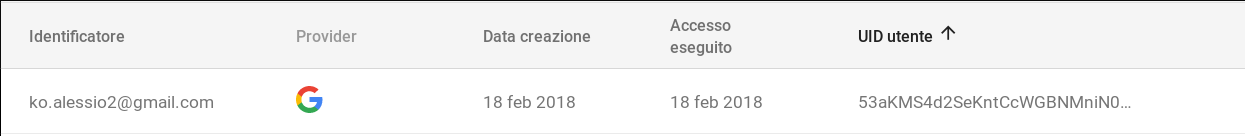
\includegraphics[width=1\textwidth]{immagini/firebase_auth_user.png}
  \caption{Schermata del pannello di controllo di FirebaseAuth User}\label{fig:Schermata del pannello di controllo di FirebaseAuth}
\end{figure}

Le informazioni salvate all'interno del servizio Firebase Auth sono differenti da quelle del database Firestore, di conseguenza per salvare ulteriori informazioni riguardanti l'utente, ogni volta che un client si registra con FirebaseAuth, verrà creato anche il suo rispettivo record all'interno del database Firestore.\\
Le informazioni aggiuntive salvate all'interno del database sono le seguenti:

\begin{itemize}
    \item \textbf{ID:} identificativo univoco assegnato dal servizio FirebaseAuth.
    \item \textbf{Name:} nome dell'utente, inserito in fase di registrazione.
    \item \textbf{Email:} email univoca di registrazione dell'utente.
    \item \textbf{PhotoUrl:} avatar opzionale dell'utente salvato su Firebase Storage.
    \item \textbf{GroupID:} gruppo di appartenenza univoco
    \item \textbf{TokenFCM:} stringa utilizzata per interagire con il servizio FCM.
\end{itemize}

\newpage



\subsection{Firestore Database}
La tipologia di database utilizzato è ``Document Based'', un database orientato agli oggetti dove i dati, a differenza dei database relazionali non vengono memorizzati in tabelle con campi uniformi per ogni record, ma ogni record è memorizzato sottoforma di documento che possiede determinate caratteristiche e può anche cambiare struttura nel tempo. Ogni documento appartiene ad una collezione, ed è memorizzato in un file JSON.\\
Il database dell'applicazione è organizzato in due sole collezioni principali, la collezione degli utenti e la collezione dei gruppi.\\
La struttura di un utente è la seguente:

\begin{table}[h]
\begin{center}
\begin{tabular}{|l|l|l|}
    \hline
\textbf{Dato} & \textbf{Tipo}  & \textbf{Descrizione}\\ \hline
ID & Int & Identificativo univoco dell'utente \\\hline
Name & String & Nome dell'utente, inserito in fase di registrazione \\ \hline
Email & String & Email univoca di registrazione dell'utente \\ \hline
PhotoUrl & String & URL dell'mmagine opzionale dell'utente \\ \hline
GroupID & Int &  Gruppo di appartenenza univoco \\ \hline
TokenFCM & String & Stringa utilizzata per interagire con il servizio FCM \\
\hline
\end{tabular}
\caption[Dati Firestore]{Strutura collezione User}\label{tab:Strutture collezione User}
\end{center}
\end{table}

L'identificativo ID assegnato all'utente è lo stesso dell'identificativo assegnato da Firebase Auth in modo da avere una diretta associazione tra il servizio Firestore e Firebase Auth.\\
Il nome, l'email e l'avatar dell'utente vengono settati attraverso le informazioni recuperate quando si esegue la registrazione tramite social login o tramite email, successivamente viene viene settato il groupID, nel momento in cui l'utente seleziona il gruppo a cui partecipare oppure sceglie di crearne uno nuovo.\\
Infine il TokenFCM è generato dall'SDK del servizio Cloud Messaging.

\newpage

L'altra collezione principale presente nel database, è la collezione che contiene i gruppi:

\begin{table}[h]
\begin{center}
\begin{tabular}{|l|l|p{9cm}|}
    \hline
\textbf{Dato} & \textbf{Tipo}  & \textbf{Descrizione}\\ \hline
ID & Int & Identificativo univoco del gruppo\\\hline
Name & String & Nome del gruppo \\ \hline
Date & Date & Data di creazione del gruppo \\ \hline
TokenFCM & String & Token utilizzato per inviare messaggi al gruppo \\ \hline
Users & Map & Oggeto che contiene la lista degli utenti del gruppo  \\ \hline
Chat & Collection &  Riferimento alla collezione Chat \\ \hline
Todolist & Collection &  Riferimento alla collezione Todolist \\ \hline
Expense & Collection & Riferimento alla collezione Expense \\
\hline
\end{tabular}
\caption[Struttura Group]{Strutture collezione Group}\label{tab:Struttura collezione Group}
\end{center}
\end{table}
L'identificativo del gruppo, la data di creazione e il nome e gli utenti appartenenti al gruppo, vengono settati al momento della creazione del gruppo, in particolare subito dopo la registrazione viene generato il ``tokenFCM'' del gruppo facendo richiesta al server FCM indicando i token di ogni dispositivo appartenente al gruppo.
Quando un utente entra all'interno di un gruppo, viene fatta richiesta al server FCM per aggiungere il token del nuovo dispositivo al gruppo, inoltre la stringa rappresentante il tokenFCM del gruppo, pur subendo cambiamenti interni, in base ai dispositivi associati ad esso, rimane invariato.\\
All'interno della collezione ``Group'' ci sono quattro subcollezioni che rappresentano le quattro funzionalità principali dell'applicazione:

\begin{itemize}
    \item \textbf{TodoList:} Contiene le mansioni del gruppo.
    \item \textbf{Expense:} Contiene le spese del gruppo.
    \item \textbf{Event:} Contiene gli eventi del gruppo.
    \item \textbf{Chat:} Contiene i messaggi del gruppo.
\end{itemize}

\newpage

All'interno della collezione ``Todolist'' sono presenti le mansioni da completare condivise nel gruppo, ogni mansione ha la seguente struttura:
\begin{table}[!h]
\begin{center}
\begin{tabular}{|l|l|p{8cm}|}
    \hline
\textbf{Dato} & \textbf{Tipo}  & \textbf{Descrizione}\\ \hline
ID & Int & Identificativo univoco della mansione \\ \hline
Name & String & Nome della mansione \\ \hline
Date & Date & Data di creazione della mansione \\ \hline
Description & String & Descrizione della mansione \\ \hline
Priority & Int & Priorità della mansione indicata con un numero da 1 a 3 \\ \hline
Members & Map & Oggetto che contiene la lista degli utenti a cui è rivolta la mansione \\ \hline
Completed\_User & String & Riferimento contenente l'UID dell'utente ha completato la mansione\\ \hline
CreatedBy & String & Riferimento contenente l'UID dell'utente ha creato la mansione \\ \hline
Status & Boolean & Booleano che indica lo stato della mansione\\
\hline
\end{tabular}
\caption[Collezione Todolist]{Struttura collezione Todolist}\label{tab:Strutture collezione Todolist}
\end{center}
\end{table}

L'identificativo di ogni mansione è assegnato dal Database Firestore, la priorità invece viene indicata sottoforma di intero, più alto è il valore dell'interno più la priorità sarà alta, e può variare da un minimo di 1 ad un massimo di 3.\\
Il campo ``status'' indica lo stato della mansione se impostato a ``false'', significa che la mansione deve essere completata, altrimenti se impostato a ``true'' significa che la mansione è stata completata, questo campo viene utilizzato dalle query per dividere le mansioni completate da quelle non completate.\\
Gli identificativi degli utenti che possono visualizzare la mansione da svolgere sono contenuti all'interno dal campo ``members'', quando un utente completa una mansione, il suo identificativo viene inserito nel campo Completed\_User, e lo stato della mansione viene impostato a ``true''.

\newpage
La seconda subcollezione contiene le spese del gruppo, la sua struttura è la seguente:
\begin{table}[!h]
\begin{center}
\begin{tabular}{|l|l|p{9cm}|}
    \hline
\textbf{Dato} & \textbf{Tipo}  & \textbf{Descrizione}\\ \hline
ID & Int & Identificativo univoco della spesa \\ \hline
Name & String & Nome della spesa \\ \hline
Date & Date & Data di scadenza della spesa \\ \hline
Description & String & Descrizione della spesa \\ \hline
Tipology & String & Tipologia della spesa \\ \hline
Members & Map & Oggetto che contiene la lista degli utenti a cui è rivolta la spesa \\ \hline
Amount & Double & Valore globale che indica l'ammontare totale della spesa effettuata \\ \hline
CreatedBy & String &  Riferimento contenente l'UID dell'utente ha creato la spesa \\ \hline
Status & Boolean & Booleano che indica lo stato della spesa\\
\hline
\end{tabular}
\caption[Collezione Spesa]{Struttura collezione Spesa}\label{tab:Strutture collezione Spesa}
\end{center}
\end{table}

L'ammontare della spesa indicata nel database è totale, quando la spesa dovrà essere divisa tra tutti gli utenti all'interno dell'oggetto ``members'', il client dovrà dividere l'ammontare totale per il numero di partecipanti alla spesa in modo da ricavare la quota parziale per ciascun utente.\\
Lo stato della spesa è globale, e può assumere valore vero o falso, se tutti gli utenti hanno pagato la loro quota, il valore di ``status'' verrà settato a ``true'' ovvero indicherà che la spesa è stata pagata da tutti.\\
La struttura dell'oggetto ``members'' è una Map chiave-valore, come chiave viene utilizzato l'identificativo UID dell'utente, mentre come valore un booleano che identifica lo stato della quota dell'utente.\\ Quando un membro del gruppo paga la sua quota il client effettua un controllo per vedere se la spesa è stata pagata da tutti o solo dall'utente.\\
Se la spesa è stata pagata solo dall'utente verrà impostato come valore della chiave dell'utente all'interno di ``members'' il valore ``true'' indicando quindi che l'utente ha pagato la spesa, altrimenti il valore della sua chiave sarà ``false''.\\
La tipologia è una stringa che permette di indicare la categoria a cui appartiene la spesa, e viene gestita lato client, con stringhe di valori predefiniti.\\


La struttura di un documento riguardante un evento invece è il seguente:
\begin{table}[!h]
\begin{center}
\begin{tabular}{|l|l|p{8cm}|}
    \hline
\textbf{Dato} & \textbf{Tipo}  & \textbf{Descrizione}\\ \hline
ID & Int & Identificativo univoco dell'evento \\ \hline
Name & String & Nome dell'evento \\ \hline
Description & String & Descrizione dell'evento \\ \hline
Date & Date & Data di creazione dell'evento \\ \hline
RecurringType & String & Stringa che indica il tipo di ricorrenza (Null, Dayly, Weekly, Monthly, Yearly) \\ \hline
Members & Map & Oggetto che contiene la lista degli utenti a cui è rivolto l'evento \\ \hline
CreatedBy & String &  Riferimento contenente l'UID dell'utente ha creato l'evento \\ \hline
\end{tabular}
\caption[Collezione Event]{Struttura collezione Event}\label{tab:Strutture collezione Event}
\end{center}
\end{table}

Il tipo di ricorrenza di un evento può assumere anche il valore ``Null'', in questo caso l'evento non sarà definito ricorrente, ma avrà una sola occorrenza stabilita dalla data inserita dall'utente.\\
Il campo ``members'' contiene invece gli utenti a cui è rivolto l'evento.


\newpage

L'ultima collezione utilizzata rappresenta i messaggi inviati all'interno della chat:


\begin{table}[h]
\begin{center}
\begin{tabular}{|l|l|p{10cm}|}
    \hline
\textbf{Dato} & \textbf{Tipo}  & \textbf{Descrizione}\\ \hline
ID & Int & Identificativo univoco del messaggio\\ \hline
Message & String & Stringa che rappresenta il contenuto del messaggio da inviare hline\\ \hline
Timestamp & Date & Data che indica il momento in cui è stato inviato il messaggio\\ \hline
SenderUID & String & Riferimento contenente l'UID dell'utente ha inviato il messaggio \\
\hline
\end{tabular}
\caption[Collezione Chat]{Struttura collezione Chat}\label{tab:Strutture collezione Chat}
\end{center}
\end{table}
La struttura è molto semplice e contiene il corpo del messaggio e la data in cui esso è stato inviato. \'E presenti anche il campo ``SenderUID'' che indica l'UID dell'utente che ha inviato il messaggio, tutti gli altri membri appartenenti al gruppo saranno automaticamente impostati come destinatari, non bisogna quindi indicare i membri del gruppo poichè la collezione chat essendo una subcollezione di groups, conosce già i componenti del gruppo.
Il valore senderUID viene anche utilizzato per impedire al server FCM di inviare una notifica se l'UID dell'utente che ha inviato il messaggio è lo stesso del nuovo messaggio inserito nel database, da un qualsiasi utente del gruppo.\\



\newpage

\subsection{Storage}
Gli utenti hanno la possibilità di salvare e personalizzare i propri avatar e gestire l'immagine del gruppo a cui appartengono, la memorizzazione di queste immagini viene fornita dal servizio Firebase Storage.
Il servizio offre la possibilità di caricare online qualsiasi tipo di file sia attraverso l'SDK sia attraverso il pannello di controllo di Firebase.\\
Ogni file presente sullo storage contiene il nome, la dimensione, il tipo e l'ultima modifica del file, oltre a queste informazioni sono presenti due link: il riferimento del file sullo storage e un URL pubblico che consente il download del file.

\begin{figure}[!hb]
  \centering
  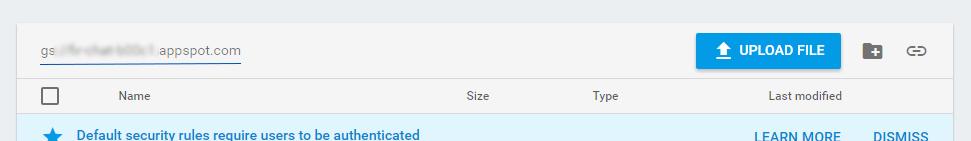
\includegraphics[width=1\textwidth]{immagini/firebase_storage.png}
  \caption{Pannello di controllo del servizio Firebase Storage}\label{fig:Pannello di controllo del servizio Firebase Storage}
\end{figure}

Il riferimento viene utilizzato dall'SDK per avere un identificativo del file all'interno dello storage, questo identificativo viene utilizzato dai client per scaricare il file applicando restrizioni di visibilità, il link pubblico invece permette a chi lo possiede di visualizzare e scaricare il file (per motivi di sicurezza questo link può essere rigenerato).\\
L'organizzazione dei file presente all'interno dello storage è gerarchica, per separare le immagini degli utenti con le immagini dei gruppi, ogni immagine viene salvata nella rispettiva cartella. Gli avatar vengono salvati all'interno della cartella ``UserAvatar'' e come nome identificativo hanno l'ID dell'utente assegnato da Firestore, le immagini dei gruppi invece vengono salvate nella cartella ``GroupAvatar'' e utilizzano come identificativo l'ID del gruppo.
Assegnando quindi come identificativo l'id dell'utente di Firestore, e l'ID del gruppo è possibile fare riferimento a tutte le immagini sia attraverso il pannello di controllo di Firebase, sia utilizzando l'SDK.\\




\subsection{Cloud Functions}
Le funzioni di Cloud Functions vengono utilizzate per inviare notifiche ai dispositivi in base a eventi scaturiti all'interno del database.

\begin{itemize}
    \item \textbf{onGroupUserAdded:} Funzione che notifica i membri di un gruppo quando viene aggiunto un nuovo utente.
    \item \textbf{onGroupExpenseAdded:} Funzione che notifica i membri di un gruppo quando viene aggiunta una nuova spesa.
    \item \textbf{onGroupTodoCompleted:} Funzione che notifica i membri di un gruppo quando viene completata una mansione.
    \item \textbf{onGroupEventAdded:} Funzione che notifica i membri di un gruppo quando viene aggiunto un nuovo evento.
    \item \textbf{onGroupTodoAdded:} Funzione che notifica i membri di un gruppo quando viene aggiunta una nuova mansione.
    \item \textbf{onGroupMessageAdded:} Funzione che notifica i membri di un gruppo quando viene inviato un messaggio nella chat.
\end{itemize}


\subsection{Cloud Messaging}
Le notifiche vengono gestite dal server Cloud Messaging, che si occupa della memorizzazione, invio e ricezioni delle notifiche fra client e server.\\
La ricezione dei messaggi da parte di Cloud Messaging è possibile solo se si utilizza l'apposito SDK e si ottiene un token, necessario per inviare un messaggio ad un dispositivo specifico, il token di registrazione viene generato automaticamente dall'SDK all'avvio dell'applicazione.\\
L'SDK consente di visualizzare i messaggi ricevuti dal servizio e gestire la generazione e il cambiamento del token. Il token di registrazione può cambiare solo quando l'applicazione viene reinstallata, disinstallata o quando vengono eliminate le cache e i dati dal dispositivo.\\
I passi necessari per connette e ricevere i messaggi dal server FCM sono i seguenti:
\begin{itemize}
    \item Client attraverso una richiesta al server FCM, richiede un token
    \item Il server FCM, se la richiesta è valida, restituisce un token di registrazione
    \item Il client invia al database Firestore il token di registrazione
    \item il client da questo momento, con il token, può inviare o ricevere messaggi connettendosi al server FCM
\end{itemize}

\begin{figure}[!hb]
  \centering
  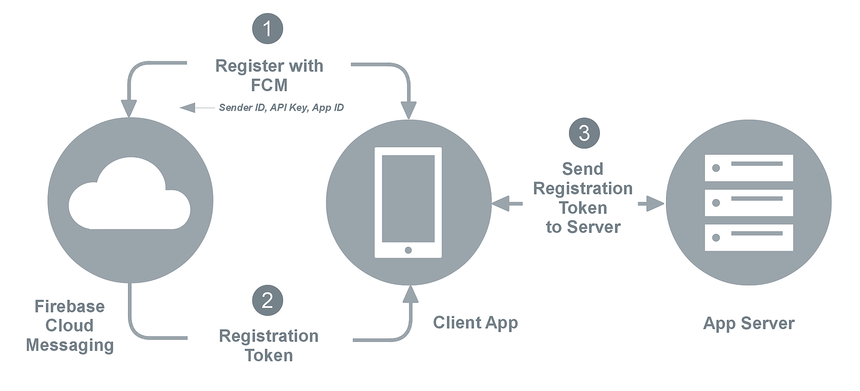
\includegraphics[width=0.65\textwidth]{immagini/fcm_token.png}
  \caption{Architettura Token FCM} \label{fig:Architettura Token FCM}
\end{figure}

\subsection{Firestore Rules}
Le regole di sicurezza Cloud Firestore Firestore Security Rules, consentono di definire norme di sicurezza per il controllo dell'accesso e la convalida dei dati.\\
La struttura del database è stata progettata per facilitare la scrittura delle regole di accesso, infatti esistono solo due collezioni principali, quella degli utenti e quella dei gruppi. Le regole di accesso dei dati sono state definite in modo tale che ogni membro del gruppo possa vedere solo i dati appartenenti al suo gruppo, in questo modo ogni mansione da svolgere, spesa, evento e messaggi all'interno della chat, sono protetti attraverso un controllo client e server.

\section{Model View Presenter}                 %crea la sezione
La parte client è stata realizzata utilizzando il pattern MVP.\\
Il MVP (Model View Presenter) è un pattern architetturale utilizzato per l'organizzazione strutturale di un progetto, in modo da trarne vantaggio in termini di prestazioni, leggibilità e modularità del codice.\\
La sua caratteristica principale è quella di separare il livello di presentazione dalla logica, in modo che tutto ciò che riguarda l'interazione dell'utente sia separato da come vengono rappresentati i dati.\\
Il pattern MVP deriva dal pattern MVC (Model View Controller), che ha 3 concetti base, che lo definiscono:

\begin{enumerate}
   \item \textbf{Model:} Il modello dei dati da visualizzare.
   \item \textbf{View:} L'interfaccia utente che visualizza i dati.
   \item \textbf{Controller:} Controlla l'interazione tra Model e View.
\end{enumerate}

La principale differenza tra i due pattern risiede nel Presenter che gestisce la logica tra la View e il Model.
Come il pattern MVC, anche il pattern MVP permette di rendere le View indipendenti dalla gestione dei dati, dividendo la logica dell' applicazione in tre livelli distinti, livelli che possono essere testati separatamente.
\begin{figure}[!b]
     \centering
     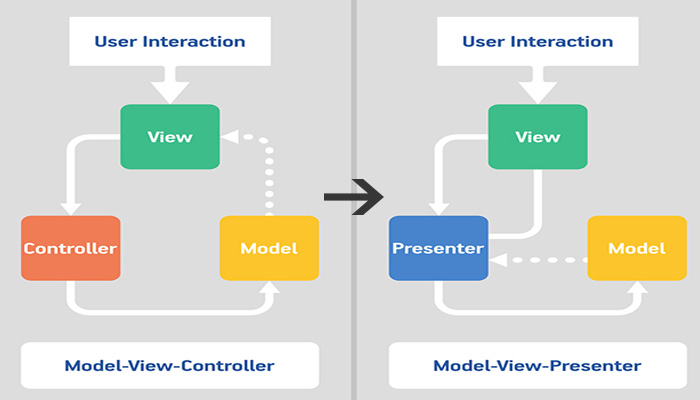
\includegraphics[width=0.65\textwidth]{immagini/mvc-vs-mvp.jpg}
     \caption{Confrontro tra il pattern MVC e MVP}\label{fig:Confrontro tra il pattern MVC e MVP}
\end{figure}

\newpage
La possibilità di poter testare i livelli separatamente è una delle caratteristiche del MVP, la sua struttur è la seguente:\@
\begin{enumerate}
   \item \textbf{Model:} Il modello è un'interfaccia che definisce i dati da visualizzare.
   \item \textbf{View:} La View è un'interfaccia passiva che visualizza i dati (il modello) e instrada i comandi utente (eventi) al Presenter per agire su tali dati.
   \item \textbf{Presenter:} Il Presenter agisce sul modello e sulla vista. Recupera i dati dai repository (il modello) e li formatta per la visualizzazione nella vista.
\end{enumerate}




\subsection{Model}
Il Model è un'interfaccia dedicata all'acceso dei dati di un'applicazione, si occupa quindi di fornire un'astrazione del modello dei dati presenti nel database.\\
Il Model oltre a contenere la struttura dei dati da visualizzare si occupa anche di fornire una buona astrazione del database, modificando, aggiungendo e separando alcuni dei dati, in modo da renderene l'accesso e la visualizzazione più semplice per gli altri due componenti del pattern (View, Presenter).\\
Un esempio potrebbe essere il seguente:
Il database contiene una tabella con due tipi di dato:

   \begin{enumerate}
   \item \textbf{Nome}: String
   \item \textbf{DataDiNascita}: Date
   \end{enumerate}

Quando il programma riceverà i dati dal database in un qualsiasi formato( Map, Json, Array) il Model selezionerà i dati in base alla definizione data dal programmatore trasformando il risultato del database in un oggetto. Questo oggetto oltre a conservare le due informazioni ricevute dal database (Nome, DataDiNascita) potrà contenere anche informazioni aggiuntive inserite dal Model per facilitare l'uso e la manipolazione degli altri due componenti.
In questo caso il modello potrebbe creare il nuovo campo ``età'' facendo una semplice sottrazione fra due date, quella attuale e la data di nascita dell'utente.

   \begin{enumerate}
   \item \textbf{Nome}: String
   \item \textbf{DataDiNascita}: Date
   \item \textbf{Età}: Int
   \end{enumerate}

   %https://medium.com/@cervonefrancesco/model-view-presenter-android-guidelines-94970b430ddf

   \subsection{View}
   La View è un'interfaccia che definisce cosa deve implementare il Presenter, affinchè possa interagire con l'interfaccia utente.\\
   La View interagisce con il Presenter per visualizzare i dati e notifica al Presenter le azioni che compie l'utente nell'interfaccia.\\
   La View può essere implementata da un Activity, un Fragment, o un widget Android, che contengono ProgressBar, TextView, RecyclerView o altri elementi che necessitano di essere aggiornati in base a qualche azione dell'utente o cambiamento nel server.\\
   Gli aggiornamenti della View possono essere gestiti in due diversi modi:
   \begin{itemize}
       \item \textbf{Passive View}
       \item \textbf{Supervising Controller}
   \end{itemize}

   Nella Passive View, il Presenter aggiorna la vista per applicare i cambiamenti del modello, in questa modalità l'interazione con il Model è gestita esclusivamente dal Presenter, la vista quindi ha un comportamento "passivo" e non è a conoscenza dei cambiamenti nel Model.\\
   Ad esempio, se si dispone di un modulo username/password e di un pulsante "Invia", non si scrive la logica di validazione all' interno della View ma all'interno del Presenter. La View infatti dovrebbe solo contenere il nome utente e la password e inviarli al Presenter.\\
   Nel Supervising Controller, la vista interagisce direttamente con il Model per eseguire semplici operazioni di binding dei dati, senza l'intervento del Presenter.
   \newpage
   Il Presenter aggiorna il Model, e gestisce cambiamenti sulla View solo nei casi più complessi, ad esempio l'aggiornamento del colore di un bordo in base alle modifiche effettuate su un dato del Model, poichè la modifica non prevede una corrispondenza diretta tra la View e il Model.
   Entrambe le modalità facilitano il testing in Android poichè le loro implementazioni riducono al minimo la quantità di logica implementata nella View.

   \begin{figure}[!hb]
     \centering
     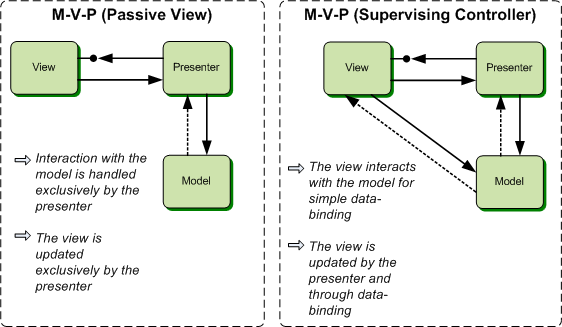
\includegraphics[width=0.7\textwidth]{immagini/mvp_view_types.png}
     \caption{MVP View types}\label{fig:Model View Types}
   \end{figure}


   \subsection{Presenter}
   Il Presenter è il mediatore tra il Model e la View e si occupa di  recuperare i dati dal Model, formattarli e passarli alla View, ma a differenza del pattern MVC, decide anche cosa succede quando si interagisce con la View reagendo alle interazioni dell'utente.\\
   Il Presenter per facilitare il testing deve cercare di non dipendere minimamente da Android, ma contenere solo metodi e dipendente Java, senza l'utilizzo del ``Context'' ad esempio.\\
   Come detto in precedenza il Presenter deve dipendere dall' interfaccia View e non direttamente dall'Activity o Fragment, in questo modo si tengono separati il Presenter e l'Activity rispettando la D dei principi SOLID: ``Dipendi dalle astensioni. Non dipendere dalle concrezioni'', questo permetterà inoltre di scrivere i test per il Presenter senza l'utilizzo di un emulatore Android.


   \section{Reactive Programming}
   La programmazione reattiva o Reactive Programming è un paradigma di programmazione che monitora e gestisce flussi di dati statici o dinamici e la propagazione dei flussi nel tempo, ciò significa che attraverso dei costrutti messi a disposizione da librerie che implementano il concetto di programmazione reattiva sarà possibile sviluppare applicazioni basate sugli eventi.\\
   Il concetto fondamentale utilizzato in questo paradigma è la possibilità di creare flussi di qualsiasi tipo sia facendo riferimento al click dell'utente sull'interfaccia grafica sia a variabili, input utente, proprietà, cache, strutture dati e richieste HTTP.\\
   Un flusso è una sequenza di eventi ordinati nel tempo che può emettere tre risposte differenti: un valore (di qualche tipo), un errore o un segnale per indicare che il flusso è terminato. Questi tre eventi vengono gestiti in modo asincrono, definendo una funzione che verrà eseguita quando verrà emesso un valore, un'altra funzione quando verà emesso un errore e un'altra funzione quando verrà completato il flusso.\\
   I due componenti principali sono quindi ``Observables'' ovvero colui che emette un flusso di dati
   e ``Observers'', ovvero colui che monitora il flusso e rimane in ascolto di nuovi valori.

   \begin{figure}[!hb]
     \centering
     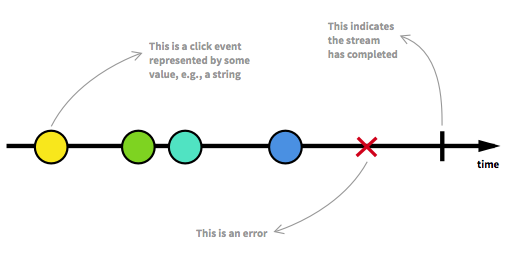
\includegraphics[width=0.65\textwidth]{immagini/reactive_programming_es1.png}
     \caption{Reactive Programming Esempio 1}\label{fig:Reactive Programming Esempio 1}
   \end{figure}

   \newpage
   \begin{itemize}
     \item \textbf{onNext}: Metodo che viene richiamato quando un Observable emette un nuovo elemento nel corso del flusso.
     \item  \textbf{OnComplete:} Metodo che indica che il flusso è giunto al termine e quindi non verrà emesso nessun nuovo elemento.
     \item \textbf{onError} Metodo che viene chiamato in presenza di errori all'interno del flusso, questo metodo interrompe il normale percorso del flusso.
   \end{itemize}

   Nello sviluppo dell'applicazione è stata utilizzata la libreria RxJava per utilizzare il paradigma di programmazione reattiva, e sfruttare la logica e i benefici della programmazione asincrona.\\
   In particolare la libreria è stata utilizzata per la gestione dei flussi di dati durante le richieste effettuate al database Firestore.

   \begin{figure}[!hb]
     \centering
     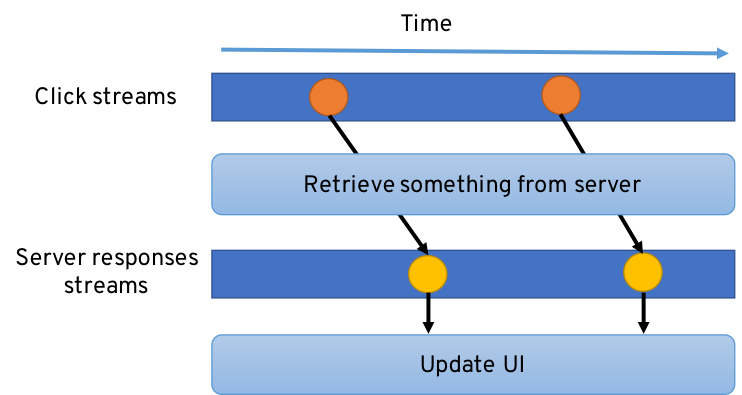
\includegraphics[width=1\textwidth]{immagini/reactive_programming_es2.png}
     \caption{Reactive Programming Esempio 2}\label{fig:Reactive Programming Esempio 2}
   \end{figure}
   
   Quando un utente si interfacciava con la pagina di una funzionalità veniva effettuata la richiesta al server e aggiornata l'interfaccia con i nuovi dati.



%%%%%%%%%%%%%%%%%%%%%%%%%%%%%%%%%%%%%%%%%non numera l'ultima pagina sinistra
\clearpage{\pagestyle{empty}\cleardoublepage}
